\documentclass[norks, final]{article}

\usepackage{notes}

\bibliography{bibliography.bib}

\author{Jon-Magnus Rosenblad}
\title{Intro til Kryptografi}

\includeonly{%
    sections/set-theory,
    sections/group-theory,
    sections/cosets,
    sections/cyclic-groups,
    sections/finite-abelian-groups,
    %sections/applications,
}

\begin{document}

\maketitle

\tableofcontents
\listoftodos

%\section{What is cryptography?}

\begin{displayquote}
    Cryptography [...] is the
\end{displayquote}


\section{Grunnleggende notasjon og mengdelære}

\begin{definition}
    En \textit{mengde} er en samling objekter $S$ hvor vi kan for
    ethvert objekt $e$ vite om $e$ tilhører $S$, skrevet $e\in S$,
    eller ikke, skrevet $e\notin S$.

    Objektene som tilhører en mengde kalles \textit{elementene}
    i mengden.
\end{definition}

Vi noterer ofte en mengde med elementene den inneholder,
til eksempel skriver vi de naturlige tallene som
\[
    \mathbb N = \{0, 1, 2, \dots\}.
\]
\begin{example}
    De naturlige tallene $\mathbb N$, heltallene $\mathbb Z$,
    de rasjonale tallene $\mathbb Q$,
    de reelle tallene $\mathbb R$
    og de komplekse tallene $\mathbb C$ danner alle mengder.

    Det finnes en tom mengde $\emptyset = \{\}$,
    og vi kan lage mengder av mengder,
    slik som mengden av den tomme mengden $\{\emptyset\}\neq\emptyset$.
\end{example}

Det finnes også samlinger av objekter som ikke danner mengder.
\begin{example}
    Samlingen av alle mengder som ikke inneholder seg selv er ikke en mengde.
    Om vi snakker om samlinger som ikke er mengder fremhever vi ofte at de ikke
    er mengder ved å bruke for eksempel klammeparenteser,
    så denne samlingen kan skrives som
    \[
        \left[
            S
            \mid
            S\notin S
        \right]
    \]
\end{example}

\begin{remark}
    Et element er enten med i en mengde eller ikke
    -- det finnes ingen id\`e om flere av det samme elementet i en mengde.
    Altså om vi har $S = \{a,b\}$, men $a = b = 1$,
    så vil $S = \{1\}$.

    Om vi vil ha flere elementer, og samtidig bryr oss om rekkefølgen av elementer
    så bruker vi en \textit{tuppel} $(a,b)$,
    så om $a = b = 1$ har vi $(a, b) = (1,1) \neq (1)$,
    men for $a\neq b$ har vi $(a, b)\neq (b, a)$.
\end{remark}

\begin{definition}
    En \textit{avbildning} $f\colon A\to B$ mellom to mengder er en
    regel som for ethvert element $a\in A$ assosierer et element
    $b = f(a)\in A$.

    Vi kaller $A$ \textit{definisjonsmengden} til $f$
    og $B$ \textit{verdimengden}.
    Vi definerer også en delmengde av $B$
    \[
        \im f = \{b\in B\mid \mbox{det finnes $a\in A$ slik at } f(a) = b\}
        \subset B
    \]
    som vi kaller \textit{bildet} av $f$.

    Vi tegner ofte opp avbildninger som piler,
    så om vi har flere mengder $A, B, C$, men flere avbildninger
    $f\colon A\to B, g\colon A\to C, h\colon B\to C$
    imellom seg kan vi tegne det opp som
    \[
        \begin{tikzcd}
            A
            \ar{rr}{f}
            \ar{rd}{g}
            &&
            B
            \ar{ld}{h}
            \\
            &
            C.
        \end{tikzcd}
    \]
\end{definition}

For ethvert element $a\in A$ finnes det bare \`en verdi for $f(a)\in B$.
Derimot kan flere verdier $a, a^\prime$ avbilde på samme verdi
$f(a) = f(a^\prime)$.

\begin{example}
    For enhver mengde $A$ finnes det en naturlig avbildning
    $\id_A\colon A\to A$ som sender hvert element $a\in A$
    på seg selv $a\mapsto a$
\end{example}

\begin{remark}
    Merk at for enhver mengde $A$ så finnes det
    nøyaktig en avbildning $\emptyset \to A$,
    men det finnes ingen avbildning $A\to \emptyset$ med mindre $A = \emptyset$.
\end{remark}

\begin{example}
    Om vi har to avbildninger $A\xrightarrow{f} B\xrightarrow{g} C$
    kan vi lage en ny avbildning $g\circ f\colon A\to C$
    ved å sende $g\circ f(a) = g(f(a))$ for alle $a\in A$.
\end{example}

\begin{definition}
    En avbildning $f\colon A\to B$ er \textit{injektiv} om for alle $a,b\in A$ med $a\neq b$
    så er $f(a)\neq f(b)$.
    Om $f$ er injektiv skriver vi ofte pilen som $f\colon A\hookrightarrow B$
    og sier at $f$ er en \textit{inklusjon}.

    Avbildningen er \textit{surjektiv} om for alle $b\in B$ så finnes en $a\in A$
    slik at $f(a) = b$.
    Om $f$ er surjektiv skriver vi noen ganger pilen som
    $f\colon A\twoheadrightarrow B$ og sier at $f$ er en \textit{surjeksjon}.

    Om $f$ er både injektiv og surjektiv sier vi den er \textit{bijektiv}
    og sier $f$ er en \textit{bijeksjon}.
\end{definition}

\begin{lemma}\label{thm:set-inverse-function}
    Om $f\colon A\to B$ er en bijeksjon så finnes en unik avbildning
    $g\colon B\to A$ slik at $f\circ g = \id_B$ og $g\circ f = \id_A$,
    dvs.
    $f(g(b)) = b$ for alle $b\in B$ og $g(f(a)) = a$ for alle $a\in A$.
    Vi kaller $g$ \textit{inversavbildningen} til $f$ og skriver $f^{-1} = g$.
\end{lemma}
\begin{proof}
    Definer en regel $g\colon B\to A$ som for hver $b\in B$ finner en $a\in A$
    slik at $f(a) = b$.
    En slik $a$ finnes alltid for enhver $b$ siden $f$ er surjektiv.

    La $g^\prime$ være en annen funksjon konstruert på samme måte,
    det vil si $g^\prime$ tilfredsstiller $f(g^\prime(b)) = b$ for alle $b\in B$.
    Men $f(g(b)) = b = f(g^\prime(b))$ og $f$ er injektiv, så $g(b) = g^\prime(b)$
    for alle $b\in B$, så $g = g^\prime$.
\end{proof}

\begin{example}
    For en mengde $A$ er $\id_A$ en bijeksjon,
    og inversavbildningen er avbildningen selv $\id_A = \id_A^{-1}$.
\end{example}

\begin{example}
    Vi kan ta \textit{snitt} og \textit{union} av mengder for å skape nye mengder.
    Snittet av to mengder $A,B$ er mengden av elementer som ligger i både $A$ og $B$
    \[
        A\cap B = \{ e\mid e\in A\mbox{ og } e\in B\},
    \]
    mens unionen er mengden av elementer i enten $A$ eller $B$
    \[
        A\cup B = \{ e\mid e\in A\mbox{ eller } e\in B\}.
    \]

    Når vi tar snitt og union følger det med naturlige inklusjoner
    \[\begin{tikzcd}
        A\cap B
        \rar[hook]
        \dar[hook]
        & B
        \dar[hook]
        \\
        A
        \rar[hook]
        &
        A\cup B
    \end{tikzcd}\].
    Disse er så naturlige at vi benevner dem som $A\cap B\subset A,B\subset A\cup B$
    utenfor diagrammer, altså er snittet $A\cap B$
    en \textit{delmengde} av $A$ (og $B$),
    og $A$ (og $B$) er en delmengde av $A\cup B$.
\end{example}

\begin{example}
    Vi har $\{1,\dots,10\}\cap \{5,\dots,15\} = \{5, 6, 7, 8, 9, 10\}$,
    og $\{1,\dots, 10,\}\cup \{5,\dots, 15\} = \{1,\dots, 15\}$.
\end{example}

\begin{definition}
    Vi kan ta \textit{komplementet} av to mengder $A, B$
    \[
        A\setminus B = \{ a\in A\mid a\notin B\} \subset A.
    \]
\end{definition}

\begin{example}
    Vi kan ta produktet av to mengder $A, B$.
    Dette er mengden
    \[
        A\times B = \{
            (a,b)\mid a\in A,\, b\in B
        \}.
    \]
    Her følger også med noen avbildninger
    \[\begin{tikzcd}
        A
        \rar[<-]{p}
        &
        A\times B
        \rar{q}
        &
        B
    \end{tikzcd}\]
    hvor $p\colon (a,b)\mapsto a$ og $q\colon (a,b)\mapsto b$ er
    projeksjonene til første og andre element henholdsvis.
\end{example}

\begin{example}
    Produktmengden til $\{0,\dots,9\}$ med seg selv består av hunder elementer,
    og vi har en bijeksjon $\{0,\dots,9\}\times\{0,\dots,9\}\to \{0,\dots,99\}$
    gitt ved $(n, m)\mapsto 10n + m$.
\end{example}

\begin{definition}
    Vi kan snakke om størrelsen på en mengde $A$ -- altså \textit{kardinaliteten}
    til mengden, som vi benevner $|A|$ eller $\# A$.
    Om $A$ inneholder et endelig antall elementer,
    så er $\# A$ antall elementer i $A$.
    Om $A$ ikke er endelig kan vi fortsatt snakke om kardinaliteten til $A$,
    og vi kan sammenligne kardinaliteter,
    for om det finnes en inklusjon $A\hookrightarrow B$
    kan vi si $\# A\leq \# B$,
    og om det finnes en bijeksjon så har vi $\# A = \# B$.
\end{definition}

\begin{example}
    Vi har
    \[
        \mathbb N
        \subset \mathbb Z
        \subset \mathbb Q
        \subset \mathbb R
        \subset \mathbb C
    \]
    så åpenbart har vi
    \[
        \#\mathbb N
        \leq \#\mathbb Z
        \leq \#\mathbb Q
        \leq \#\mathbb R
        \leq \#\mathbb C,
    \]
    men det viser seg at
    \[
        \#\mathbb N
        = \#\mathbb Z
        = \#\mathbb Q
        < \#\mathbb R
        = \#\mathbb C.
    \]
    Merk at $\mathbb Z$ og $\mathbb R$ har forskjellig kardinalitet,
    men begge er uendelige.
    Vi benevner den første uendeligheten med $\aleph_0 = \#\mathbb Z$,
    og den sistnevnte som $\aleph_1 = \#\mathbb R$.
\end{example}

\begin{example}
    La $A, B$ være to mengder.
    Vi kan lage mengden av alle avbildninger fra $A$ til $B$
    \[
        \mathrm{Map}(A,B) = \{f\colon A\to B\}.
    \]
    Vi sier to avbildninger $f,g\colon A\to B$
    er like om $f(a) = g(a)$ for alle $a\in A$.
\end{example}

\subsubsection*{Oppgaver}

\begin{enumerate}
    \item Vis at om $f\colon A\hookrightarrow B$ er en injeksjon
        så finnes en $g\colon B\twoheadrightarrow A$ slik at
        $g\circ f = \id_A$.
        Er den unik?
    \item La $A\xrightarrow{f} B\xrightarrow{g} C$ være to avbildninger.
        \begin{enumerate}
            \item
                Anta $g\circ f$ er surjektiv.
                Vis at da må $f$ være surjektiv.
            \item
                Anta $g\circ f$ er injektiv.
                Vis at da må $f$ være injektiv.
            \item
                Om $g\circ f$ er en bijeksjon, må $f$ eller $g$ være en bijeksjon?
        \end{enumerate}
    \item La $U$ være en mengde, og $A, B\subset U$ to delmengder.
        Vis identiteten
        \[
            U\setminus(A\cap B) = (U\setminus A)\cup (U\setminus B).
        \]
    \item La $A, B$ være to endelige mengder, og la $n = \# A$ og $m=\# B$,
        vis at da er $\# \mathrm{Map}(A,B) = m^n$.
        Dette motiverer hvorfor flere forfattere velger å skrive
        $\mathrm{Map}(A,B) = B^A$.
    \item La $\mathrm{Bij}(A)$ benevne mengden av bijeksjoner $s\colon A\to A$,
        og la $f\colon A\to B$ være en bijeksjon.
        Vis at avbildningen $\tilde f\colon \mathrm{Bij}(A)\to \mathrm{Bij}(B)$
        gitt ved $s\mapsto f\circ s\circ f^{-1}$ er en bijeksjon.
\end{enumerate}
Mengdeteoretisk definerer vi ofte en avbildning $A\to B$ som en samling data
$(A, B, \Gamma)$ med $\Gamma\subset A\times B$ slik at for alle $a\in A$
så finnes en unik $b\in B$ slik at $(a,b)\in \Gamma$.
Denne delmengden $\Gamma$ kalles \textit{grafen} til funksjonen,
for om vi skal gi den tilhørende ``regelen'' $f$ får vi $f(a) = b$
for alle $(a,b)\in \Gamma$.

\begin{remark}
    Merk at for en $A\to B$ er både $A$ og $B$ del av
    dataen, så for to avbildninger $f, g$ med definisjonsmengde
    $A$ og samme graf $\Gamma_f = \Gamma_g$ så kan de være forskjellige
    om de har forskjellige verdimengder $B_f, B_g$,
    til eksempel om $B_g\subsetneq B_f$.
\end{remark}
\begin{example}
    La $f\colon \mathbb Z\to \mathbb Z$ og
    $g\colon \mathbb Z\to 2\mathbb Z$
    hvor
    \[
        2\mathbb Z = \{2n \mid n\in \mathbb Z\}\subset \mathbb Z.
    \]
    Både $f$ og $g$ er gitt ved $f(n) = g(n) = 4n$ for alle $n\in \mathbb Z$,
    så de har samme bilde i $\im f = \im g\subset\mathbb Z$,
    men de har forskjellig verdimengde, så $f\neq g$.
\end{example}
\begin{enumerate}[resume]
    \item
        \begin{enumerate}
            \item Hva betyr det for $\Gamma$ at $f$ er injektiv?
            \item Hva betyr det for $\Gamma$ at $f$ er surjektiv?
            \item Kan du bevise \cref{thm:set-inverse-function} på en annen
                måte ved å bruke denne nye definisjonen av en avbildning?
        \end{enumerate}
\end{enumerate}

\begin{figure}[htb]
    \centering
    \begin{subfigure}[b]{.3\textwidth}
        \centering
        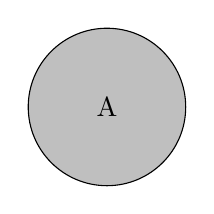
\begin{tikzpicture}
            \draw[fill=lightgray] (0,0) circle (1);
            \draw (0,0) node {A};
        \end{tikzpicture}
        \caption{En mengde $A$}
    \end{subfigure}
    \begin{subfigure}[b]{.3\textwidth}
        \centering
        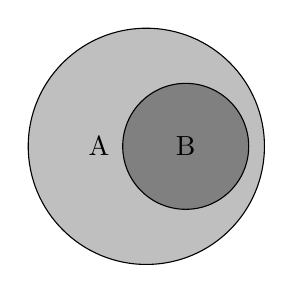
\begin{tikzpicture}
            \draw[fill=lightgray] (0,0) circle (1.5);
            \draw[fill=gray] (.5,0) circle (.8);
            \draw (-.6,0) node {A};
            \draw (.5, 0) node {B};
        \end{tikzpicture}
        \caption{$B\subset A$}
    \end{subfigure}
    \begin{subfigure}[b]{.3\textwidth}
        \centering
        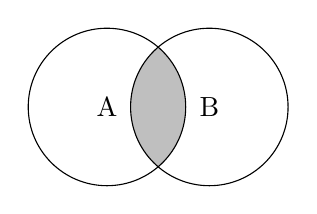
\begin{tikzpicture}
            \coordinate (a) at (0,0);
            \coordinate (b) at (1.3, 0);
            \begin{scope}
                \clip (b) circle (1);
                \fill[lightgray] (a) circle (1);
            \end{scope}
            \draw (a) node{A} circle(1);
            \draw (b) node{B} circle(1);
        \end{tikzpicture}
        \caption{$A\cap B$}
    \end{subfigure}
    \begin{subfigure}[b]{.3\textwidth}
        \centering
        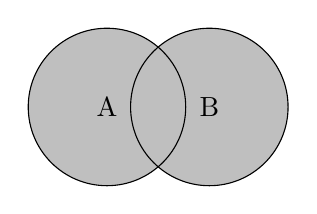
\begin{tikzpicture}
            \coordinate (a) at (0,0);
            \coordinate (b) at (1.3, 0);
            \fill[lightgray] (a) circle (1)
                (b) circle (1);
            \draw (a) node{A} circle(1);
            \draw (b) node{B} circle(1);
        \end{tikzpicture}
        \caption{$A\cup B$}
    \end{subfigure}
    \begin{subfigure}[b]{.3\textwidth}
        \centering
        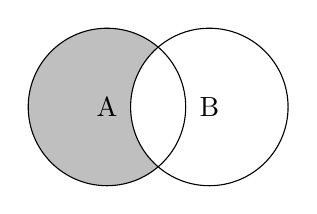
\begin{tikzpicture}
            \coordinate (a) at (0,0);
            \coordinate (b) at (1.3, 0);
            \begin{scope}[even odd rule]
                \clip (a) circle (1) (b) circle (1);
                \fill[lightgray] (a) circle (1);
            \end{scope}
            \draw (a) node{A} circle(1);
            \draw (b) node{B} circle(1);
        \end{tikzpicture}
        \caption{$A\setminus B$}
    \end{subfigure}
    \begin{subfigure}[b]{.38\textwidth}
        \centering
        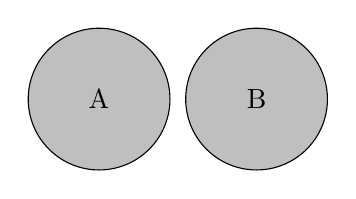
\begin{tikzpicture}
            \coordinate (a) at (0,0);
            \coordinate (b) at (2, 0);
            \draw[fill=lightgray] (a) node{A} circle(.9);
            \draw[fill=lightgray] (b) node{B} circle(.9);
        \end{tikzpicture}
        \caption{$A\cap B=\emptyset$}
    \end{subfigure}
    \caption{Konsepter om mengder.}
\end{figure}

\begin{figure}
    \centering
    \begin{subfigure}[b]{.49\textwidth}
        \centering
        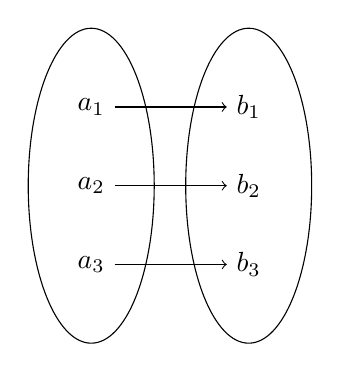
\begin{tikzpicture}
            \begin{scope}
                \draw (0,0) node (a1) {$a_1$}
                    ++(0,-1) node (a2) {$a_2$}
                    ++(0,-1) node (a3) {$a_3$};
                \draw (a2) ellipse (.8 and 2);
            \end{scope}
            \begin{scope}[xshift=2cm]
                \draw (0,0) node (b1) {$b_1$}
                    ++(0,-1) node (b2) {$b_2$}
                    ++(0,-1) node (b3) {$b_3$};
                \draw (b2) ellipse (.8 and 2);
            \end{scope}
            \draw[->] (a1) -- (b1);
            \draw[->] (a2) -- (b2);
            \draw[->] (a3) -- (b3);
        \end{tikzpicture}
        \caption{En bijeksjon.}
    \end{subfigure}
    \begin{subfigure}[b]{.49\textwidth}
        \centering
        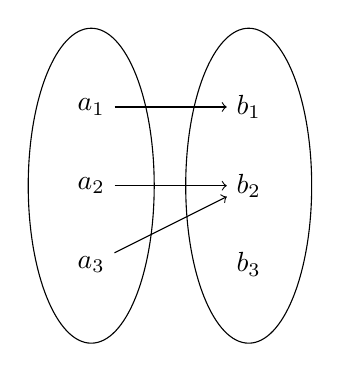
\begin{tikzpicture}
            \begin{scope}
                \draw (0,0) node (a1) {$a_1$}
                    ++(0,-1) node (a2) {$a_2$}
                    ++(0,-1) node (a3) {$a_3$};
                \draw (a2) ellipse (.8 and 2);
            \end{scope}
            \begin{scope}[xshift=2cm]
                \draw (0,0) node (b1) {$b_1$}
                    ++(0,-1) node (b2) {$b_2$}
                    ++(0,-1) node (b3) {$b_3$};
                \draw (b2) ellipse (.8 and 2);
            \end{scope}
            \draw[->] (a1) -- (b1);
            \draw[->] (a2) -- (b2);
            \draw[->] (a3) -- (b2);
        \end{tikzpicture}
        \caption{Hverken en injeksjon eller surjeksjon.}
    \end{subfigure}
    \begin{subfigure}[b]{.49\textwidth}
        \centering
        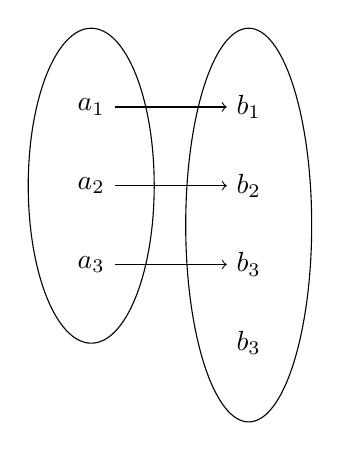
\begin{tikzpicture}
            \begin{scope}
                \draw (0,0) node (a1) {$a_1$}
                    ++(0,-1) node (a2) {$a_2$}
                    ++(0,-1) node (a3) {$a_3$};
                \draw (a2) ellipse (.8 and 2);
            \end{scope}
            \begin{scope}[xshift=2cm]
                \draw (0,0) node (b1) {$b_1$}
                    ++(0,-1) node (b2) {$b_2$}
                    ++(0,-1) node (b3) {$b_3$}
                    ++(0,-1) node (b4) {$b_3$};
                \path (b2) -- (b3) coordinate[midway] (c){};
                \draw (c) ellipse (.8 and 2.5);
            \end{scope}
            \draw[->] (a1) -- (b1);
            \draw[->] (a2) -- (b2);
            \draw[->] (a3) -- (b3);
        \end{tikzpicture}
        \caption{En injeksjon.}
    \end{subfigure}
    \begin{subfigure}[b]{.49\textwidth}
        \centering
        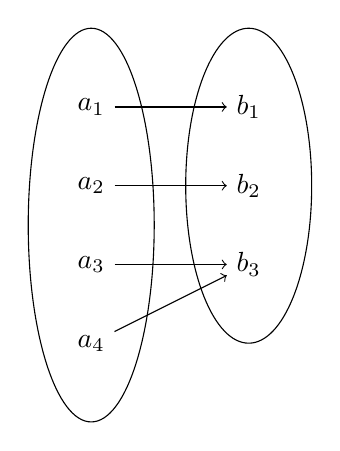
\begin{tikzpicture}
            \begin{scope}
                \draw (0,0) node (a1) {$a_1$}
                    ++(0,-1) node (a2) {$a_2$}
                    ++(0,-1) node (a3) {$a_3$}
                    ++(0,-1) node (a4) {$a_4$};
                \path (a2) -- (a3) coordinate[midway] (c);
                \draw (c) ellipse (.8 and 2.5);
            \end{scope}
            \begin{scope}[xshift=2cm]
                \draw (0,0) node (b1) {$b_1$}
                    ++(0,-1) node (b2) {$b_2$}
                    ++(0,-1) node (b3) {$b_3$};
                \draw (b2) ellipse (.8 and 2);
            \end{scope}
            \draw[->] (a1) -- (b1);
            \draw[->] (a2) -- (b2);
            \draw[->] (a3) -- (b3);
            \draw[->] (a4) -- (b3);
        \end{tikzpicture}
        \caption{En surjeksjon.}
    \end{subfigure}
    \caption{Konsepter om avbildninger.}
\end{figure}

\subsection{Mengdelære i kryptografi}

Mengdelære er et veldig fundamentalt område innen matematikken,
men enda kan vi bruke noen av disse primitive redskapene til å si noe om
kryptografiske metoder.

Vi har sett fire kategorier av kryptografiske metoder,
nemlig
\begin{itemize}
    \item hashing,
    \item symmetrisk kryptering,
    \item asymmetrisk kryptering, og
    \item nøkkelutveksling.
\end{itemize}
Disse kan alle beskrives som avbildninger,
og vi kan allerede si at disse avbildningene må tilfredsstille visse egenskaper,
men først må vi definere mengdene disse avbildningene avbilder imellom.

Ofte er det tre mengder vi har i tankene,
\begin{itemize}
    \item $\mathscr M$ -- mengden av meldinger som Alice og Bob kan tenke seg å
        sende.
        Dette kan være mengden av alle tekster som kan tenkes og skrives,
        eller det kan være en forhåndsbestemt mengde av bare et fåtall uttrykk,
        slik som $\{\mathrm{Ja}, \mathrm{Nei}\}$.
    \item $\mathscr K$ -- mengden av nøkler som kan velges av Alice og Bob.
    \item $\mathscr C$ -- mengden av mulige chiffertekster.
\end{itemize}

\subsubsection{Hash-funksjoner}
En hashfunksjon i generell forstand er bare en avbildning $h\colon \mathscr M\to \mathscr C$.
Ofte ønsker vi noe som heter en \textit{perfekt} hash som vil si at om vi har to forskjellige
meldinger $m\neq m^\prime\in \mathscr M$ så hashes meldingene til forskjellige
chiffertekster $h(m)\neq h(m^\prime)\in \mathscr C$.
I kryptografi er det ofte tilstrekkelig at det ikke er ``for mange'' meldinger
som har samme chiffertekst,
men vi stiller ofte andre strenge krav til hvordan chifferteksten skal
skille seg mellom ulike meldinger.

\subsubsection{Symmetrisk kryptering}
En symmetrisk krypteringsalgoritme er to avbildninger
$f\colon \mathscr M\times \mathscr K\to \mathscr C$
og $g\colon \mathscr C\times \mathscr Kt\to \mathscr M$
slik at for alle $m\in \mathscr M$ og $k\in \mathscr K$
har vi $g(f(m, k),k) = m$.
Om vi velger en fast nøkkel $k\in \mathscr K$ kan vi definere
to nye funksjoner
\[
    f_k\colon \begin{cases}
        \mathscr M\to \mathscr C
        \\
        m\mapsto f(m, k)
    \end{cases}
\]
og
\[
    g_k\colon \begin{cases}
        \mathscr C\to \mathscr M
        \\
        c\mapsto g(c, k),
    \end{cases}
\]
så $g_k\circ f_k = \id_{\mathscr M}$.
Spesielt betyr dette at $f_k$ må være injektiv,
og $g_k$ blir dermed surjektiv.

\subsubsection{Asymmetrisk kryptering}
En asymmetrisk algoritme er nesten  det samme,
men nå kan vi tenke oss at $f$ og $g$ bruker
bare delvis informasjon om nøkkelen.
Nå kan vi tenke oss en nøkkel $k\in\mathscr K$ som et par
$k = (k_a, k_b)$ hvor $k_a\in \mathscr K_a$ velges blant
en mengde private nøkler,
og $k_b\in \mathscr K_b$ velges blant en mengde offentlige nøkler,
så $\mathscr K\subset \mathscr K_a\times\mathscr K_b$.

Nå blir de to funksjonene gitt ved
\[\begin{aligned}
    f&\colon\mathscr M\times \mathscr K_a\to \mathscr C\\
    g&\colon\mathscr C\times \mathscr K_b\to \mathscr M
\end{aligned}\]
slik at $g_{k_b}\circ f_{k_a} = \id_{\mathscr M}$.
Det som er viktig her er at $(k_a, k_b)$ alltid opptrer i par
slik at for hver $k_a\in\mathscr K_a$ finnes en unik $k_b\in\mathscr K_b$
slik at $g_{k_b}\circ f_{k_a} = \id_{\mathscr M}$ og visa versa.
Det følger at vi har en bijeksjon $\mathscr K_a\to\mathscr K_b$
som for hver private nøkkel gir den tilhørende offentlige nøkkelen,
men denne bijeksjonen må være umulig å beregne for at algoritmen skal være sikker.
Merk at $\mathcal K\subset \mathcal K_a\times \mathcal K_b$ er grafen til denne bijeksjonen.
For at algoritmen skal være brukbar må det derimot være mulig å trekke tilfeldige
nøkkelpar $(k_a, k_b)$ fra $\mathcal K$.

\subsubsection{Nøkkelutveksling}
I klassisk Diffie-Hellman er algoritmen for Alice og Bob identisk,
så vi har to funksjoner
\[\begin{aligned}
    f&\colon \mathscr K\times\mathscr K\to \mathscr K
    \\
    g&\colon \mathscr K\to \mathscr K
\end{aligned}\]
slik at om Alice velger en nøkkel $k_a$ og Bob en nøkkel $k_b$
har vi $f(k_a, g(k_b)) = f(k_b, g(k_a))$.
Her er $g(k_a$ Alice sin offentlige nøkkel som hun deler med Bob,
og $g(k_b)$ er Bob sin offentlige nøkkel som han deler med Alice.
For algoritmens sikkerhet er det viktig at man ikke kan regne ut
$k$ fra $g(k)$, og at gitt $g(k_a)$ og $g(k_b)$
kan vi ikke regne ut $f(k_a, g(k_b))$.

\section{Grunnleggende gruppeteori}

\begin{definition}
    En \textit{gruppe} $(G,\ast)$ er en mengde $G$ sammen med en avbildning
    $\ast\colon G\times G\to G$.
    For to elementer $g, h\in G$ skriver vi $\ast(g,h)$ som $g\ast h$.
    Paret $(G, \ast)$ må tilfredsstille at
    \begin{itemize}
        \item det finnes et element $e\in G$ hvor for alle $g\in G$
            har vi $e\ast g = g\ast e = g$.
            Dette elementet er unikt med denne egenskapen (vis dette!)
            og kalles \textit{identitetselementet} $e_G = e \in G$.
        \item for $g, h, i\in G$ har vi
            $g\ast (h\ast i) = (g\ast h)\ast i$,
            altså $\ast$ er \textit{assosiativ}, og
        \item for hver $g$ finnes et element $h\in G$
            slik at $g \ast h = e$.
            Dette elementet $h$ er unikt med denne egenskapen (vis dette!)
            og vi benevner det $h = g^{-1}$, \textit{inverselementet}.
    \end{itemize}
    Vi sier at $\ast$ er \textit{gruppeoperatoren} til gruppen $(G,\ast)$.
\end{definition}

For å gjøre notasjonen enklere skriver vi ofte bare $G$ for gruppen $(G,\ast)$
når gruppeoperatoren er åpenbar.
Vi forkorter ofte også $g\ast h$ som $gh$.

\begin{definition}
    En avbildning $f\colon G\to H$ mellom to grupper
    er en \textit{morfi} om
    \begin{itemize}
        \item $f(e_G) = e_H$, og
        \item for alle $g, g^\prime\in G$ har vi $f(gg^\prime) = f(g)f(g^\prime)$.
    \end{itemize}
\end{definition}

\begin{definition}
    En delmengde $H\subset G$ av en gruppe $(G, \ast)$ er en \textit{undergruppe}
    om
    \begin{itemize}
        \item $e\in H$,
        \item for alle $h, h^\prime \in H$ er $h\ast h^\prime\in H$,
            og
        \item for alle $h\in H$ er $h^{-1}\in H$.
    \end{itemize}
\end{definition}

\begin{remark}
    Inklusjonen av en undergruppe $H\subset G$
    \[
        H\hookrightarrow G
    \]
    er en morfi.
\end{remark}

\begin{example}
    Vi kjenner allerede til mange eksempler på grupper,
    slik som kjeden av delmengder
    \[
        \mathbb Z
        \subset \mathbb Q
        \subset \mathbb R
        \subset \mathbb C
    \]
    hvor vi lar $\mathbb C = (\mathbb C, +)$ være en gruppe under addisjon
    danner en kjede av undergrupper.
    Merk at $\mathbb N$ ikke er en gruppe under addisjon siden det ikke finnes
    invers elementer.

    Om vi fjerner $0$ fra alle mengdene
    \[
        \mathbb Q^\times
        \subset \mathbb R^\times
        \subset \mathbb C^\times
    \]
    og utruster $\mathbb C$ med multiplikasjon isteden,
    så danner dette en kjede med undergrupper.
\end{example}

\begin{example}
    Om $(G, \ast_G), (H, \ast_H)$ er to grupper så danner $(G\times H, \ast)$
    en gruppe hvor $\ast$ er operatoren
    \[
        (g, h)\ast (g^\prime, h^\prime)
        = (g \ast_G g^\prime, h\ast_H h^\prime).
    \]
    Til eksempel er det reelle planet $\mathbb R^2$ en gruppe under vektor-addisjon.
\end{example}

\begin{example}
    La $\mathrm{Bij}(A)$ være mengden av bijeksjoner $A\to A$.
    Da er $(\mathrm{Bij}(A), \circ)$ en gruppe.
\end{example}

\begin{example}
    Mengden $\mathrm{Mat}_{2\times 2}$ av $(2\times 2)$-matriser under addisjon
    danner en gruppe.
\end{example}

\begin{example}
    Mengden $\mathrm{GL}_2(\mathbb R)$ av inverterbare $(2\times2)$-matriser
    med koeffisienter i $\mathbb R$
    danner en gruppe under matrise multiplikasjon.
\end{example}

\begin{example}
    La $f\colon G\to H$ være en morfi.
    Husk at for en avbildning definerte vi bildet av avbildningen
    $\im f\subset H$ som en delmengde.
    Denne delmengden er også en undergruppe.
\end{example}

La $f\colon G\to H$ være en morfi.
I tillegg til bildet $\im f\subset H$ kan vi lage en annen undergruppe.
\begin{definition}
    Vi definerer \textit{kjernen} til $f\colon G\to H$
    som
    \[
        \ker f = \{ g\in G\mid f(g) = e_H\} \subset G.
    \]
\end{definition}

\begin{lemma}
    Kjernen $\ker (f\colon G\to H)\subset G$ av en morfi er en undergruppe av $G$.
\end{lemma}
\begin{proof}
    Vi trenger å vise at $e_G\in \ker f$, at $\ker f$ er lukket under
    gruppe-operatoren, og at det finnes inverser.
    Den førstnevnte følger fra at $f(e_G) = e_H$ siden $f$ er en morfi.

    La $g,g^\prime \in\ker f$, da har vi $f(g) = f(g^\prime) = e_H$,
    men $f(gg^\prime) = f(g)f(g^\prime) = e_H$, så $gg^\prime\in \ker f)$.

    La $g\in \ker f$, så $f(g) = e_H$, men $f(g^{-1}) = {f(g)}^{-1} = e_H$,
    så $g^{-1}\in\ker f$.
\end{proof}

\begin{definition}
    La $(G, \ast_G), (H, \ast_H)$ være to grupper.
    Vi kan definere en operator $\ast_{G\times H}$
    på $G\times H$ ved
    \[
        (g, h)\ast_{G\times H} (g^\prime, h^\prime)
        = (g \ast_G g^\prime, h \ast_H h^\prime).
    \]
    Dette gjør $G\times H$ til en gruppe med identitetselement $(e_G, e_H)$.
\end{definition}

Som med mengder har vi fortsatt de to projeksjonene
\[\begin{tikzcd}
    G
    \rar[<-]{p}
    &
    G\times H
    \rar{q}
    &
    H,
\end{tikzcd}\]
men vi har også inklusjoner den andre veien
\[\begin{tikzcd}
    G
    \rar{\id_G\times e_H}
    &
    G\times H
    \rar[<-]{e_G\times \id_H}
    &
    H,
\end{tikzcd}\]
gitt ved $(\id_G\times e_H)\colon g\mapsto (g, e_H)$
og $(e_G\times \id_H)\colon h\mapsto (e_G, h)$.
Disse tilfredsstiller $p\circ (\id_G\times e_H) = \id_G$
og $q\circ (e_G\times \id_H) = \id_H$.
Merk også at $\im (\id_G\times e_H) = \ker q$.

\subsubsection*{Oppgaver}
\begin{enumerate}
    \item Finn enhetselementet og inverselementene til alle eksemplene på
        grupper nevnt ovenfor.
    \item Vis at det bare finnes ett element $e\in G$ slik
        at $e \ast g = g\ast e = g$ for alle $g\in G$,
        altså at identitetselementet er unikt.
    \item Vis at for enhver $g\in G$ så finnes det bare ett element
        $h\in G$ slik at $gh = e$.
    \item Vis at for en morfi $f\colon G\to H$
        så har vi for alle $g\in G$ at $f(g^{-1}) = {f(g)}^{-1}$.
    \item Vis at for en morfi $f\colon G\to H$ så er $\im f\subset H$ en undergruppe.
\end{enumerate}
Så langt har vi sett mange eksempler på uendelige grupper,
slik som $\mathbb C$ og dens undergrupper.
Vi ønsker å se på flere eksempler av \textit{endelige} grupper,
det vil si grupper hvor den underliggende mengden er endelig.
\begin{enumerate}[resume]
    \item La $S^1\subset \mathbb C$ være enhetsirkelen
        \[
            S^1 = \{ z\in \mathbb C\mid |z| = 1\}.
        \]
        \begin{enumerate}
            \item Vis at $S^1$ er en gruppe under (kompleks) multiplikasjon.
            \item La $n$ være et heltall og la $\mu_n\subset S^1$ være mengden av $n$-te
                enhetrøtter
                \[
                    \mu_n = \{
                        e^{\frac k n 2\pi i}
                        \mid k\in \mathbb Z
                    \}.
                \]
                Vis at $\# \mu_n = n$ og at $\mu_n$ er en delgruppe av $S^1$.
            \item Ta for deg $\mu_3, \mu_4$ og $\mu_{12}$.
                Vis at $f\colon \mu_{12}\to \mu_3\times \mu_4$
                gitt ved
                \[
                    e^{\frac k {12} 2\pi i}
                    \mapsto (e^{\frac k 3 2\pi i}, e^{\frac k 4 2\pi i})
                \]
                er en isomorfi.

                Det finnes en slik isomorfi $\mu_{nm}\to \mu_n\times \mu_m$
                så lenge $\mathrm{gcd}(n,m) = 1$.
            \item Vis at det ikke finnes noen isomorfi $\mu_4\to \mu_2\times\mu_2$.
        \end{enumerate}
    \item Ta for deg gruppen $\mathrm{Bij}(S)$ av bijeksjoner $S\to S$
        hvor $S$ er en endelig mengde.
        Vi så at om vi har en bijeksjon $f\colon S\to S^\prime$
        så er avbildningen
        $\tilde f\colon \mathrm{Bij}(S)\to \mathrm{Bij}(S^\prime)$
        gitt ved $\sigma\mapsto f\circ \sigma \circ f^{-1}$
        for hver $(\sigma\colon S\to S)\in\mathrm{Bij}(S)$
        en bijeksjon.
        \begin{enumerate}
            \item Vis at $\tilde f$ er en morfi.
                Det følger dermed at at $\tilde f$ er en isomorfi.
            \item Vis (ved induksjon) at om $S, S^\prime$ er to endelige mengder
                slik at $\# S = \# S^\prime$.
                Da finnes det en bijeksjon $S\to S^\prime$.
        \end{enumerate}
        Vi har nå sett at om to endelige mengder $S, S^\prime$
        har samme antall elementer så er gruppene av bijeksjoner
        $\mathrm{Bij}(S), \mathrm{Bij}(S^\prime)$ isomorfe.
        La $n = \# S$.
        Vi gir denne gruppen det generelle navnet
        \textit{gruppen av permutasjoner av $n$ elementer}
        $S_n = \mathrm{Bij}(\{1,\dots,n\})$.
        \begin{enumerate}[resume]
            \item Vis at $\# S_n = n!$.
        \end{enumerate}
    \item La $G$ være en endelig gruppe.
        En nært beslektet mengde til $S_n$ er mengden
        $\mathrm{Aut}(G) = \mathrm{Iso}(G, G)$
        av isomorfier $G\to G$, såkalte \textit{automorfier} av $G$.
        \begin{enumerate}
            \item Vis at $(\mathrm{Aut}(G), \circ)$ er en gruppe.
            \item Vis at om en bijeksjon $f\colon G\to H$ er en isomorfi,
                så er $\tilde f\colon \mathrm{Aut}(G)\to \mathrm{Aut}(H)$
                en isomorfi.
            \item Vis at $\mathrm{Aut}(\mu_4)$ ikke er isomorf
                med $\mathrm{Aut}(\mu_2\times\mu_2)$.
                [Merk at $\#\mathrm{Aut}(\mu_4) = 2$.]
        \end{enumerate}
\end{enumerate}



\section{Restklasser}

\begin{definition}
    La $H\subset G$ være en undergruppe.
    En \textit{restklasse} av $H$ i $G$ er en mengde på formen
    \[
        gH = \{gh\mid h\in H\}
    \]
    for en $g\in H$.
    Merk at $g\in gH$ siden $e\in H$.
\end{definition}

\begin{example}
    La $G = \mathbb Z$ være gruppen av heltall under addisjon.
    Ta for deg undergruppen $H = 2\mathbb Z = \{ 2n\mid n\in \mathbb Z\}$
    av partall.
    Partallene har to restklasser i $\mathbb Z$,
    nemlig mengden vi får når vi legger til et partall $2m$
    \[
        2m + (2H) = \{2m + 2n = 2(m + n)\mid n\in \mathbb Z\} = 2\mathbb Z
    \]
    som blir partallene selv,
    og mengden vi får når vi legger til et oddetall
    \[
        (2m + 1) + (2H) = \{2m + 1 + 2n
        = 2(m + n) + 1\mid n\in \mathbb Z\} = 1 + 2\mathbb Z
    \]
    som blir alle oddetallene.
\end{example}

\begin{lemma}
    La $g, g^\prime$ være to elementer i $G$,
    og la $H\subset G$ være en undergruppe av $G$.
    Vi har
    \[
        gH = g^\prime H
    \]
    hvis og bare hvis $g^{-1} g^\prime\in H$.
\end{lemma}
\begin{proof}
    Anta at $g H = g^\prime H$,
    så for alle $h\in H$ finnes en $h^\prime\in H$
    slik at $gh = g^\prime h^\prime$,
    men da kan vi regne
    \[\begin{aligned}
        gh &= g^\prime h^\prime \\
        g^{-1} gh = h
           &= g^{-1} g^\prime h^\prime \\
        h {(h^\prime)}^{-1}
           &= g^{-1} g^\prime h^\prime {(h^\prime)}^{-1}
            = g^{-1} g^\prime
    \end{aligned}\]
    så $g^{-1}g^\prime = h {(h^\prime)}^{-1}\in H$ siden $H$ er en undergruppe.

    For den andre veien anta at $g^{-1} g^\prime \in H$.
    Anta for motsigelse at $gH\neq g^\prime H$,
    så ved symmetri kan vi anta (``uten tap av generalitet'')
    at det finnes et element $gh\in gH$
    slik at $gh\notin g^\prime H$.
    Men $g^{-1} g^\prime \in H$,
    så $h^\prime = {(g^{-1} g^\prime)}^{-1} h\in H$,
    så $gh = g (g^{-1}g^\prime) h^\prime = g^\prime h^\prime \in g^\prime H$,
    men vi antok at $gh\notin g^\prime H$, så vi har en motsigelse.
\end{proof}

\begin{corollary}\label{thm:coset-no-partial-intersection}
    Om $gH\cap g^\prime H\neq \emptyset$ så har vi $gH = g^\prime H$.
\end{corollary}

\begin{corollary}
    Restklassene til $H\subset G$ danner en \textit{partisjon} av $G$,
    det vil si vi kan finne en \textbf{delmengde} (ikke en gruppe) elementer
    $S\subset G$ slik at $gH \cap g^\prime H = \emptyset$ for alle $g,g^\prime\in S$
    med $g\neq g^\prime$, og
    \[
        \bigcup_{g\in S} gH = G.
    \]
\end{corollary}
\begin{proof}
    La $\mathscr S$ være mengden delmengder $S\subset G$ slik at
    for alle $g,g^\prime \in G$ så har vi $gH\cap g^\prime = \emptyset$
    for $g\neq g^\prime$.
    Anta $\tilde S\in \mathscr S$ er maksimal, det vil si det finnes ingen
    $S\in \mathscr S$ slik at $\tilde S\subsetneq S$.
    Vi påstår at $\bigcup_{g\in \tilde S} gH = G$.
    Anta for motsigelse at det finnes en $g^\prime\in G$ slik at
    $g^\prime\notin \bigcup_{g\in \tilde S} gH$.
    Da har vi at $g^\prime H\cap gH = \emptyset$ for alle $g\in \tilde S$,
    for ellers har vi $g^\prime \in gH$ ved \cref{thm:coset-no-partial-intersection},
    men da har vi at $\tilde S\cup \{g^\prime\}\in\mathscr S$
    som motsier at $\tilde S$ er maksimal,
    så det finnes ingen slik $g^\prime$ og $\bigcup_{s\in\tilde S} gH = G$.
\end{proof}

\begin{remark}
    Hvordan vet vi egentlig at det i det hele tatt finnes en maksimal
    mengde $\tilde S$ i $\mathscr S$?
    Om gruppen er uendelig kan man tenke seg at vi alltid
    har plass til å legge til flere og flere elementer til $\tilde S$.
    Det som redder oss er at vi vet at $\tilde S$ er ihvertfall mindre enn $G$,
    så vi kan på en litt innviklet måte bruke et ganske abstrakt aksiom
    kalt \textit{Zorns lemma} til å vite at det finnes et maksimalt element,
    men vi vet ikke nødvendigvis hvordan vi skal finne et slikt element!
\end{remark}

\subsection{Kvotientgruppen}

\begin{lemma}
    La $G$ være en gruppe, $H\subset G$ en undergruppe
    og $g\in G$ et element.
    Da er $\# gH = \# H$.
\end{lemma}
\begin{proof}
    Vi har en naturlig avbildning $f\colon H\to gH$ gitt ved $h\mapsto gh$.
    Denne er surjektiv per definisjon av $gH$, så det gjenstår å vise at den er
    injektiv.

    Anta at $f(h) = f(h^\prime)$ for to $h, h^\prime \in H$,
    altså at $gh = gh^\prime$, men da har vi at
    \[
        h
        = g^{-1} f(h)
        = g^{-1} f(h^\prime)
        = h^\prime.
    \]
\end{proof}

\begin{definition}
    La $G$ være en gruppe og $H\subset G$ en undergruppe.
    Vi definerer mengden av restklasser
    \[
        G / H = \{ gH \mid g\in G\}.
    \]
\end{definition}

\begin{remark}
    Merk at avbildningen $G\to G / H$ gitt ved $g\mapsto gH$ ikke er injektiv,
    for det er flere ulike $g\neq g^\prime$ slik at $gH = g^\prime H$,
    og dette er akkurat de parene $(g, g^\prime)$ slik at $g^{-1}g^\prime\in H$.
\end{remark}

\begin{example}
    La $H\subset G$ være endelige grupper.
    Vi har allerede sett at restklassene danner en partisjon av $G$,
    og nå har vi sett at alle restklassene er like store.
    Det følger umiddelbart at vi må ha
    \[
        \# G = \# (G / H) \# H,
    \]
    altså
    \[
        \# G / \# H = \# (G / H)
    \]
    som motiverer notasjonen.
\end{example}

Vi kan tenke oss en naturlig gruppeoperator på mengden $G / H$,
nemlig at for to restklasser $gH$ og $g^\prime H$ definerer vi produktet deres som
\[
    (gH)(g^\prime H) = (gg^\prime)H,
\]
men husk at vi har flere elementer $\hat g\in G$ som gir samme restklasse
$\bar gH = gH$ enda $\bar g\neq g$.
Så for at denne operatoren skal være ``veldefinert'' på $G / H$ trenger
vi at $(\bar gg^\prime) H = (g g^\prime)H$,
det vil si at
${(g g^\prime)}^{-1} (\bar g g^\prime) = {(g^\prime)}^{-1} h g^\prime\in H$
hvor $h = g^{-1} g\in H$,
men dette er ikke automatisk!

\begin{example}
    Ta for deg gruppen av permutasjoner $G = S_3$ av mengden på tre elementer $\{1,2,3\}$,
    og la $H$ være undergruppen bestående av identiteten og permutasjonen
    \[
        (12)\colon \begin{cases}
            1\mapsto 2\\
            2\mapsto 1\\
            3\mapsto 3.
        \end{cases}
    \]
    La $g= (13)$ og $g^\prime (23)$.
    Vi ser at $gH = \{(13)e, (13)(12)\} = \{(13), (123)\}$,
    så $\bar gH = gH$ hvor $\bar g = (123)$,
    men $gg^\prime = (13)(23) = (321)$,
    mens $\bar g g^\prime = (123)(23) = (12)$,
    så
    \[
        (gg^\prime)H = (321)H\neq H = (12)H = (\bar g g^\prime)H.
    \]
\end{example}

\begin{definition}
    En undergruppe $H\subset G$ er \textit{normal}
    dersom
    \[
        gH = Hg = \{hg\mid h\in H\}
    \]
    for alle $g\in G$.
\end{definition}

\begin{lemma}
    Om $H\subset G$ er en normal undergruppe så er ``multiplikasjon''
    veldefinert på mengden av restklasser $G / H$,
    så $G / H$ danner en gruppe -- \textit{kvotientgruppen} av $G$ over $H$.
\end{lemma}
\begin{proof}
    Om vi har $gH = Hg$ for alle $g\in H$ så følger det at
    $H = g^{-1} H g$,
    så $g^{-1}h g\in H$ for alle $h\in H$.
\end{proof}

\begin{lemma}
    La $f\colon G\to H$ være en morfi.
    Da er $\ker f\subset G$ en normal undergruppe.
\end{lemma}
\begin{proof}
    La $vg\in(\ker f) g$.
    Vi ønsker å vise at $vg\in g\ker f$,
    men det er det samme som at $g^{-1} vg\in \ker f$.
    Vi ser at
    \[\begin{aligned}
        f(g^{-1}vg)
        &= f(g^{-1})f(v)
        \\
        &= {(f(g))}^{-1} e_H f(g)
        \\
        &= e_H,
    \end{aligned}\]
    så $g^{-1} vg\in \ker f$.
\end{proof}

\begin{theorem}
    La $f\colon G\to H$ være en surjektiv morfi.
    Da har vi en isomorfi $\hat f\colon G / \ker f \to H$,
    det vil si vi kan fylle inn følgende avbildning
    \[\begin{tikzcd}
        G
        \rar
        \drar[swap]{f}
        &
        G / \ker f
        \dar[dashed]{\bar f}
        \\
        &
        H.
    \end{tikzcd}\]
\end{theorem}
\begin{proof}
    Vi benevner restklassen $g + \ker f$ i $G / \ker f$
    ved $\bar g$.
    Vi konstruerer en avbildning $\bar f\colon G / \ker f\to H$
    ved at for en $\bar g\in G / \ker f$ setter vi
    $\bar f(\bar g) = f(g)$ for en representant $g$.

    Om vi velger en annen representant $g^\prime$ med
    $\bar g^\prime = \bar g$ har vi at $g^{-1}g^\prime\in\ker f$,
    så $f(g) = f(g)f(g^{-1}g^\prime) = f(gg^{-1})f(g^\prime) = f(g^\prime)$,
    så definisjonen av $\bar f$ er uavhengig av hvordan vi velger representanter.

    For alle $h\in H$ så finnes en $g\in G$ slik at $f(g) = h$,
    så $\bar f(\bar g) = h$, og $\bar f$ er surjektiv.

    \todo[inline]{Vis injektivitet og at det er en morfi}
\end{proof}

\subsubsection*{Oppgaver}

\begin{enumerate}
    \item
        \begin{enumerate}
            \item Hvilke restklasser har $3\mathbb Z = \{3n \mid n\in \mathbb Z\}$
                i $\mathbb Z$? Hva med $5\mathbb Z\subset \mathbb Z$?
            \item For et generelt heltall $n\in \mathbb Z$,
                vis at $n\mathbb Z\subset \mathbb Z$ har $n$ restklasser,
                det vil si $\#(\mathbb Z / n\mathbb Z = n$.
        \end{enumerate}
    \item Bevis \cref{thm:coset-no-partial-intersection}
    \item Vi skal undersøke mengden av restklasser til $\mathbb Z\subset \mathbb R$.
        \begin{enumerate}
            \item Vi har sett at to restklasser $a + \mathbb Z = b + \mathbb Z$
                hvis og bare hvis $(a - b)\in \mathbb Z$.
                Bruk dette til å konstruere en bijeksjon
                $[0,1)\to \mathbb R / \mathbb Z$.
            \item Vi har at $a + \mathbb Z = \mathbb Z + a$,
                så $\mathbb Z\subset \mathbb R$ er en normal undergruppe
                og $\mathbb R / \mathbb Z$ danner en gruppe.
                Vis at avbildningen
                \[
                    \mathrm{exp}\colon \begin{cases}
                        (\mathbb R, +)\mapsto (S^1,\times)\\
                        x\mapsto e^{2\pi i x}
                    \end{cases}
                \]
                er en gruppe-morfi (merk at vi går fra addisjon til multiplikasjon)
                og at den danner en bijeksjon $[0,1)\to S^1$.
                Her er $S^1$ enhetsirkelen
                \[
                    S^1 = \{z\mid |z| = 1\}\subset \mathbb C.
                \]
                Dette viser at vi har en isomorfi $\mathbb R / \mathbb Z \to S^1$.
            \item Kan du forestille deg hva som skjer om vi tar
                $\mathbb R / \mathbb Q$?
        \end{enumerate}
\end{enumerate}


\section{Sykliske grupper}

\begin{definition}
    En gruppe $(G, \ast)$ er \textit{abelsk} om
    for alle $g,h\in G$ har vi $g\ast h = h\ast g$.
    En operator som tilfredsstiller dette kalles \textit{kommutativ}.
\end{definition}

\begin{example}
    Alle eksemplene er med addisjon som gruppeoperator ovenfor er abelske.
    Generelt, om vi benevner en operator med symbolet ``$+$'' så er operatoren
    kommutativ.
\end{example}

\begin{example}
    Gruppen av invertible $(2\times 2)$-matriser under multiplikasjon
    $\mathrm{GL}_2(\mathbb R)$
    er ikke abelsk, siden til eksempel
    \[
        \begin{bmatrix}
            1 & 1\\
            0 & 1
        \end{bmatrix}
        \begin{bmatrix}
            1 & 0\\
            1 & 1
        \end{bmatrix}
        =
        \begin{bmatrix}
            1 & 1\\
            1 & 2
        \end{bmatrix}
    \]
    mens
    \[
        \begin{bmatrix}
            1 & 0\\
            1 & 1
        \end{bmatrix}
        \begin{bmatrix}
            1 & 1\\
            0 & 1
        \end{bmatrix}
        =
        \begin{bmatrix}
            2 & 1\\
            1 & 1
        \end{bmatrix}.
    \]
\end{example}

\begin{definition}
    La $g_1,\dots, g_n\subset G$ være et endelig antall elementer i $G$.
    Vi definerer \textit{gruppen generert av $g_1,\dots, g_n$}
    \[
        H = \langle g_1,\dots,g_n\rangle \subset G
    \]
    som den minste undergruppen av $G$ som inneholder alle elementene $g_1,\dots,g_n$.

    Om det finnes en $g\in G$ slik at $G = \langle g\rangle$ sier vi at $G$
    er en \textit{syklisk} gruppe.
\end{definition}

\begin{example}
    Heltallene $\mathbb Z$ er en syklisk gruppe generert av $1$.
    Alle undergruppene $n\mathbb Z\subset \mathbb Z$ er også sykliske generert av
    $n$.
\end{example}

\begin{lemma}\label{thm:cyclic-surjection}
    La $G$ være en gruppe.
    Da er $G$ syklisk hvis og bare hvis det finnes en surjektiv morfi
    $\mathbb Z\to G$.
\end{lemma}
\begin{proof}
    Anta det finnes en surjektiv avbildning $f\colon \mathbb Z\to G$.
    Da har vi at for alle $g\in G$ så finnes en $n\in \mathbb Z$ slik at
    $f(n) = f(1)^n = g$, så $G = \langle f(1)\rangle$.

    Anta at $G = \langle g \rangle$ for en $g\in G$.
    Vi konstruerer en avbildning $f\colon \mathbb Z\to G$
    gitt ved $n\mapsto g^n$.
    Åpenbart har vi at $\im f\subset G$,
    men $\im f$ er en undergruppe av $G$ og $g\in \im f$,
    så $\langle g\rangle\subset \im f$ siden $\langle g\rangle$
    er den minste undergruppen som inneholder $g$.
    Men $\langle g\rangle = G$,
    så dermed har vi at $\langle g \rangle = \im f = G$,
    så $f$ er surjektiv.
\end{proof}

\begin{corollary}\label{thm:integer-subgroups}
    Undergruppene $k\mathbb Z = \langle k\rangle \subset \mathbb Z$
    er de eneste undergruppene $\mathbb Z$ har.
\end{corollary}
\begin{proof}
    La $k_1, \dots, k_n$ være en endelig samling elementer i $\mathbb Z$.
    Da finnes det heltall $c_1,\dots,c_n$ slik at $c_1 k_1 + \dots + c_n k_n = k$
    hvor $k = \mathrm{gcd}(k_1,\dots,k_n)$
    er største felles nevner for $k_1,\dots, k_n$.
    Dette følger fra Euclids algoritme.
    Da vil $\langle k_1,\dots, k_n\rangle = \langle k\rangle$.

    Et tilsvarende argument holder for uendelige samlinger $\{k_i\}$
    ved å velge en endelig delmengde.
\end{proof}

\begin{corollary}
    La $G$ være en syklisk gruppe.
    Da finnes en isomorfi $\mathbb Z / n\mathbb Z\to G$
    hvor $n = \# G$.
\end{corollary}
\begin{proof}
    Siden $G$ er syklisk finnes en surjektiv morfi $f\colon \mathbb Z\to G$
    ved \cref{thm:cyclic-surjection}.
    Vi har at $\ker f\subset \mathbb Z$ er en undergruppe,
    så det finnes en $n\in \mathbb Z$ slik at
    $\ker f = n\mathbb Z$ ved \cref{thm:integer-subgroups},
    så $\bar f\colon \mathbb Z / \ker f = \mathbb Z / n\mathbb Z\to G$
    er en isomorfi.
    Merk at en isomorfi er en bijeksjon, så $\# G = \# \mathbb Z / n\mathbb Z = n$.
\end{proof}

\begin{remark}
    De endelige gruppen $\mathbb Z / n\mathbb Z$ er en slags ``modell''
    for alle sykliske grupper av $n$ elementer,
    så vi kommer til å bruke den mye og skriver ofte bare
    \[
        \mathbb Z / n = \mathbb Z / n\mathbb Z.
    \]
\end{remark}

\begin{example}
    Enhetrøttene $\mu_n$ er en syklisk gruppe,
    så vi har en isomorfi $\mathbb Z / n \to \mu_n$.
\end{example}

\begin{theorem}[Kinesisk restteorem]\label{thm:chinese-remainder}
    La $n\in \mathbb Z$ og la $k_1,\dots, k_r\in \mathbb Z$ være en rekke heltall.
    Vi har naturlige morfier $f_i\colon \mathbb Z\to \mathbb Z / k_i$
    for alle $i=1,\dots,r$.
    La $n_i$ være restklassen til $n$ i $\mathbb Z / k_i$.
    Da har vi at $f_i(n^\prime) = n_i$ for alle $i=1,\dots,r$
    hvis og bare hvis $n - n^\prime\in k\mathbb Z$ hvor
    \[
        k
        = \mathrm{lcm}(k_1,\dots,k_r)
        = \frac {k_1\dots k_n}{\mathrm{gcd}(k_1,\dots,k_n)}.
    \]
\end{theorem}
\begin{proof}
    Siden
    $\mathrm{lcm}(k_1,\dots,k_r)
    = \mathrm{lcm}(k_1, \mathrm{lcm}(k_2,\dots,k_r))$
    viser vi resultatet ved induksjon på $r$.

    Om $r = 1$ er $\mathrm{lcm}(k_1) = k_1 = k$,
    så resultatet er umiddelbart.

    Før vi går videre observerer vi at vi kan omformulere teoremet
    ved hjelp av diagrammet
    \[\begin{tikzcd}
        \mathbb Z
        \rar
        \drar[swap]{f_1\times \dots\times f_r}
        &
        \mathbb Z / \mathrm{lcm}(k_1,\dots,k_r)
        \dar{\bar f_1\times\dots\times\bar f_r}
        \\
        &
        (\mathbb Z / k_1)\times \dots\times(\mathbb Z / k_r).
    \end{tikzcd}\]
    Teoremet sier at om vi har et element
    $(n_1,\dots,n_r)\in (\mathbb Z / k_1)\times\dots\times(\mathbb Z / k_r)$
    i bildet av $f_1\times\dots\times f_r)$
    så finnes en unik restklasse $n + (k\mathbb Z)$ slik at
    \[
        (\bar f_1\times\dots\times \bar f_r)(n + (k\mathbb Z)) = (n_1,\dots, n_r),
    \]
    altså har vi en isomorfi
    \[
        \mathbb Z / k\xrightarrow{\sim} \im (f_1\times\dots\times f_2).
    \]
    Tanken er at vi filtrerer dette bildet
    \[\begin{tikzcd}
        \mathbb Z
        \ar[bend right]{ddddr}
        \rar
        &
        \mathbb Z / \mathrm{lcm}(k_1,\dots,k_r)
        \dar
        \\
        &
        (\mathbb Z / k_1) \times (\mathbb Z / \mathrm{lcm}(k_2,\dots, k_r))
        \dar
        \\
        &
        (\mathbb Z / k_1)
        \times (\mathbb Z / k_2)
        \times (\mathbb Z / \mathrm{lcm}(k_3,\dots, k_r))
        \dar
        \\
        &
        \dots
        \dar
        \\
        &
        (\mathbb Z / k_1)
        \times\dots\times (\mathbb Z / k_r).
    \end{tikzcd}\]

    Anta at $f_i(n^\prime) = n_i$ for alle $i=2,\dots, r$ hvis og bare
    hvis $n^\prime - n\in k^\prime \mathbb Z$ hvor
    $k^\prime = \mathrm{lcm}(k_2,\dots,k_r)$.
    Anta også at $f_1(n^\prime) = n_1$.
    Da har vi at
    \[
        n = n_1 + k_1 m_1 = n^\prime + k^\prime m_2
    \]
    og $n^\prime = n_1 + k_1 m_1^\prime$,
    så
    \[
        n - n^\prime = k_1 (m_1 - m_1^\prime) = k^\prime m_2.
    \]
    Merk at $k_1 | n - n^\prime$,
    og $k^\prime | n - n^\prime$,
    så $\mathrm{lcm}(k_1, k^\prime) = k | n - n^\prime$,
    så $n - n^\prime \in k\mathbb Z$.
\end{proof}

\subsubsection*{Oppgaver}
\begin{enumerate}
    \item La $A$ være en abelsk gruppe og $H\subset A$ en undergruppe.
        \begin{enumerate}
            \item Vis at $H$ er abelsk.
            \item Vis at $H$ er en normal undergruppe.
        \end{enumerate}
    \item La $n, m$ være heltall.
        Vi har sett at om $m\mid n$ så finnes en injeksjon
        $\mathbb Z / m \hookrightarrow \mathbb Z / n$
        som identifiserer $\mathbb Z / m$ som en undergruppe av $\mathbb Z / n$.
        \begin{enumerate}
            \item Vis at dersom $\mathrm{gcd}(n, m) = 1$ så er den eneste morfien
                $\mathbb Z / m \to \mathbb Z / n$ den som sender hele
                $\mathbb Z / m$ på $0$.
            \item Vis at dersom $\mathrm{gcd}(n, m) = d$ så kan alle morfier
                $f\colon \mathbb Z / m \to \mathbb Z / n$ faktoriseres som
                \[
                    \mathbb Z / m
                    \xrightarrow{g} \mathbb Z / d
                    \xhookrightarrow{i} \mathbb Z / n,
                \]
                det vil si $f$ kan skrives som $f = i\circ g$.
        \end{enumerate}
        La $G$ være en gruppe. En \textit{ekte} undergruppe $H \subset G$
        er en undergruppe slik at $H\neq \{e_H\}$ og $H\neq G$.
        \begin{enumerate}[resume]
            \item Vis at $\mathbb Z / p$ ikke har noen ekte undergrupper.
                En gruppe uten ekte undergrupper kalles en \textit{simpel} gruppe.
        \end{enumerate}
\end{enumerate}
Ta for deg en endelig syklisk gruppe $\mathbb Z / n\mathbb Z$.
Multiplikasjon gir oss en avbildning
$\mu\colon \mathbb Z\times \mathbb Z\to \mathbb Z$
gitt ved $(a,b)\mapsto ab$.
Om vi tar $a^\prime, b^\prime$ slik at
$a^\prime - a, b^\prime - b\in n\mathbb Z$,
det vil si at det finnes $k, l\in \mathbb Z$ slik at
$a^\prime = a + kn$ og $b^\prime = b + lb$,
så har vi at
\[\begin{aligned}
    \mu(a^\prime, b^\prime)
    &= \mu(a + kn, b + ln)
    \\
    &= (a + kn)(b + ln)
    \\
    &= ab + (al + bk + kln)n
    \\
    &= \mu(a, b) + (al + bk + kln)n,
\end{aligned}\]
så $\mu(a^\prime, b^\prime) - \mu(a, b) \in \mathbb Z$.
Det følger at vi kan lage en morfi $\hat\mu$ som passer i diagrammet
\[\begin{tikzcd}
    \mathbb Z\times \mathbb Z
    \rar{\mu}
    \dar
    &
    \mathbb Z
    \dar
    \\
    (\mathbb Z / n\mathbb Z)\times(\mathbb Z / n\mathbb Z)
    \rar{\hat\mu}
    &
    \mathbb Z,
\end{tikzcd}\]
altså kan vi definere multiplikasjon på $\mathbb Z / n\mathbb Z$ også.
\begin{enumerate}[resume]
    \item Vis at om $\mathrm{gcd}(a, n) = d$ så finnes det en
        $b$ slik at $\bar\mu(a, b) = d\in \mathbb Z / n\mathbb Z$.
        Spesielt om $n = p$ er et primtall så finnes det for alle
        \[
            a \in (\mathbb Z / p\mathbb Z)\setminus\{0\}
            = {(\mathbb Z / n\mathbb Z)}^\times
        \]
        et element $b\neq 0$ slik at $\overline\mu(a, b) = 1$,
        det vil si at multiplikasjon $\bar\mu$ på
        ${(\mathbb Z / p\mathbb Z)}^\times$ har inverselementer,
        så $({(\mathbb Z / p\mathbb Z)}^\times, \bar\mu)$ danner en gruppe.
    \item Vi benevner $\bar\mu$ ovenfor som $\times$ og skriver
        $\bar\mu(a,b)$ bare som $ab$.
        Vis at $({(\mathbb Z / p\mathbb Z)}^\times, \times)$ er syklisk,
        så
        \[
            ({(\mathbb Z / p\mathbb Z)}^\times, \times)
            \cong (\mathbb Z / (p - 1)\mathbb Z, +).
        \]
\end{enumerate}
\begin{remark}
    Denne isomorfien er viktig for flere kryptografiske algoritmer,
    slik som Diffie-Hellman,
    for selv om det ser ut som vi jobber over gruppen $\mathbb Z / p\mathbb Z$,
    så jobber vi over den multiplikativt.
    Det handler i prinsipp om at vi jobber over ${(\mathbb Z / p\mathbb Z)}^\times$
    slik at vi har en komplisert måte å jobbe med $\mathbb Z / (p - 1)\mathbb Z$.
\end{remark}

Selv om $n$ ikke er et primtall kan vi definere en gruppe under multiplikasjon
som en del av $\mathbb Z / n\mathbb Z$.
La
\[
    {(\mathbb Z / n\mathbb Z)}^\times
    = \{ a\mid \mathrm{gcd}(a, n) = 1\}.
\]
Merk at denne definisjonen sammenfaller med vår
tidligere definisjon når $n$ er et primtall.
\begin{enumerate}[resume]
    \item La $n = p_1\dots p_r$ være en faktorisering av $n$
        slik at $p_i$ er primtall for alle $i=1,\dots,r$.
        Vis at $\# {(\mathbb Z / n\mathbb Z)}^\times = (p_1 - 1)\dots(p_r - 1)$.
\end{enumerate}

\section{Endelige abelske grupper}

\subsection{Fermats lille teorem}

\begin{lemma}\label{thm:binomial-identity}
    La $x,y\in \mathbb Z$  og $n \geq 1$ være heltall.
    Da har vi formelen
    \[
        (x + y)^n = \sum_{i = 0}^n \binom n i x^i y^{n - i}.
    \]
\end{lemma}

Av og til tar vi dette som definisjonen av \textit{binomialkoeffisientene}
$\binom n m$,
men om vi heller bruker definisjonen fra Pascals trekant $\binom n 0 = \binom n n = 1$
for alle $n\in\mathbb N$ og $\binom n {m - 1} + \binom n m = \binom {n + 1} m$
for alle $n, m$ kan vi vise \cref{thm:binomial-identity} ved induksjon som følger.
\begin{proof}
    Tilfellet $n = 1$ er enkelt siden
    $(x + y)^1 = x + y$ og $\binom 1 0 = \binom 1 1 = 1$.

    Anta $(x + y)^k = \sum_{i = 0}^k \binom k i x^i y^{k - i}$.
    Vi har
    \[\begin{aligned}
        (x + y)^{k + 1}
        &=  (x + y)(x + y)^k
        \\
        &= (x + y)\sum_{i = 0}^k \binom k i x^i y^{k - i}
        \\
        &= \sum_{i = 0}^k \binom k i x^{i + 1} y^{k - i}
        + \sum_{i = 0}^k \binom k i x^{i} y^{k - i + 1}
        \\
        &= \sum_{i = 1}^{k + 1} \binom k {i - 1} x^{i} y^{(k + 1) - i}
        + \sum_{i = 0}^k \binom k i x^{i} y^{(k + 1) - i}
        \\
        &= \sum_{i = 0}^{k + 1} \binom {k + 1} i x^{i} y^{(k + 1) - i}
    \end{aligned}\]
\end{proof}

\begin{corollary}{Fermats lille teorem}
    La $p$ være et primtall.
    Da har vi at
    \[
        a^p \cong a \mod p
    \]
    for alle $a\in \mathbb Z$.
\end{corollary}
\begin{proof}
    Vi definerer en avbildning $\pi_p\colon \mathbb Z / p\to\mathbb Z / p$
    ved $a\mapsto a^p$.
    La $a,b\in \mathbb Z$.
    Vi ser at
    \[\begin{aligned}
        \pi_p(a + b)
        &= (a + b)^p
        \\
        &= \sum_{i = 0}^p \binom p i a^i b^{p - i}
        \\
        &= a^p + b^p
        \\
        &= \pi_p(a) + \pi_p(b)
    \end{aligned}\]
    siden $p|\binom p i$ for $i\neq 0, p$,
    så $\pi_p$ er en morfi.
    Vi ser også at $\pi_p(1) = 1^p = 1$,
    og det er bare \`en morfi $\mathbb Z / p\to \mathbb Z / p$
    som tilfredsstiller dette, nemlig identiteten $\id_{\mathbb Z / p}$,
    så $\pi_p = \id_{\mathbb Z / p}$.
\end{proof}

\subsection{Klassifisering av endelige abelske grupper}
Vi har allerede sett at alle endelige sykliske grupper kan skrives på formen
$\mathbb Z / n$ for et heltall $n$.
Vi ønsker å generalisere dette til alle endelige abelske grupper.
Vi har sett at det finnes endelige abelske grupper som ikke er sykliske
slik som $\mathbb Z / 2\times \mathbb Z / 2$ og genereres av minst to elementer.
Andre grupper som vi genererer av to elementer kan vise seg å være sykliske derimot,
slik som $\mathbb Z / 2\times \mathbb Z / 3 \cong \mathbb Z / 6$.
Som en konsekvens av \cref{thm:chinese-remainder} kan vi vise
\begin{corollary}\label{thm:cyclic-refactoring}
    La $p_1,\dots,p_n$ være primtall slik at $p_i \neq p_j$
    for alle $i\neq j$,
    og la $r_1,\dots,r_n$ være heltall.
    Da har vi en isomorfi
    \[
        \mathbb Z / (p_1^{r_1}\dots p_n^{r_n})
        \cong
        \mathbb Z / p_1^{r_1}\times\dots\times\mathbb Z / p_n^{r_n}.
    \]
\end{corollary}

Vi ønsker noe i denne stilen som tar hånd om alle endelige abelske grupper.

\begin{lemma}\label{thm:cycles-divide-maximal}
    La $A$ være en endelig abelsk gruppe og la $\langle a\rangle$
    være en syklisk undergruppe av maksimal orden.
    La $\langle a^\prime\rangle$ være en annen syklisk undergruppe.
    Da $\#\langle a^\prime\rangle | \#\langle a\rangle$.
\end{lemma}
\begin{proof}
    La $l$ være det minste positive heltallet slik at
    $\langle a\rangle \cap \langle a^\prime \rangle = \langle la^\prime\rangle$.
    La $m = \#\langle a\rangle$, $n = \#\langle a^\prime\rangle$,
    og $d = \mathrm{gcd}(m, l)$.
    Merk at $\frac n l = \#\langle la^\prime\rangle$.
    Da har vi $\mathrm{gcd}(m, l / d) = 1$,
    men $\#\langle \frac {nd} l a^\prime\rangle = l / d$,
    så
    \[
        a\in \langle \frac l d a\rangle
        \subset \langle a + \frac {nd} l a^\prime\rangle,
    \]
    men $\langle a\rangle$ er maksimal,
    så $l = d$ og $\frac {nd} l a^\prime = na^\prime = 0$.
    Det følger også at $l | m$, så $n = l\frac n l | m$.
\end{proof}

\begin{corollary}
    Let $a, a^\prime\subset A$ slik at $\langle a\rangle$
    er en maksimal syklisk undergruppe.
    Da finnes $a^{\prime\prime}$ slik at
    \[
        \langle a, a^\prime\rangle
        = \langle a, a^{\prime\prime}\rangle,
    \]
    men $\langle a\rangle \cap \langle a^{\prime\prime}\rangle = 0$.
\end{corollary}
\begin{proof}
    La $l$ være det minste positive heltallet slik at
    $\langle a\rangle \cap \langle a^\prime\rangle = \langle la^\prime\rangle$.
    La $k$ være det minste helltallet slik at $ka = la^\prime$.
    La $n = \# \langle a\rangle$ og $m = \#\langle a^\prime\rangle$,
    så $m | n$ siden $\langle a\rangle$ er maksimal.
    Vi har også at $\frac n l la^\prime = \frac n l ka = 0$,
    så $m | \frac n l k$.
    Siden $n | m$ følger det at $\frac m n | \frac k l$, så $l | k$.
    La $a^{\prime\prime} = a^\prime - \frac m l a$.
    Vi har $a^\prime \in \langle a, a^{\prime\prime}\rangle$.

    La $s$ være det minste positive heltallet slik at
    $sa^{\prime\prime}\in \langle a\rangle$,
    så $sa^\prime - s\frac m l a\in \langle a \rangle$,
    men da må $sa^\prime\in\langle a\rangle$,
    så $s = l$ og $sa^{\prime\prime} = 0$.
    Det følger at $\langle a\rangle \cap \langle a^{\prime\prime}\rangle = 0$.
\end{proof}

\begin{lemma}\label{thm:free-surjection}
    La $A = \langle a_1,\dots,a_k\rangle$ være en abelsk gruppe.
    Da har vi en surjektiv morfi
    \[
        \phi\colon\mathbb Z^k\to A
    \]
    gitt ved $e_i\mapsto a_i$ for alle $i=1,\dots,k$.
\end{lemma}
\begin{proof}
    Merk at $\phi$ er en morfi og $a_i\in \im\phi$,
    så $\langle a_1,\dots,a_k\rangle\subset \im\phi\subset A$,
    så $\phi$ er surjektiv.
\end{proof}

\begin{corollary}\label{thm:maximal-cycle-split}
    La $A$ være en endelig abelsk gruppe og $a\in A$
    et element slik at $\langle a\rangle$ er en maksimal syklisk undergruppe.
    Da har inklusjonen $\iota \colon \langle a\rangle\to A$ en venstre invers
    $\rho\colon A\to \langle a\rangle$,
    det vil si $\rho\circ \iota = \id$.
    Det følger at vi har en isomorfi
    \[
        A = \langle a\rangle \times (A / \langle a\rangle).
    \]
\end{corollary}
\begin{proof}
    La $\langle a_1,\dots, a_k$ være et valg av generatorer for $A$.
    For hver $i = 1,\dots,k$ velg en $a_i^\prime$
    slik at $\langle a\rangle\cap \langle a_i^\prime\rangle = 0$
    og $a_i \in \langle a, a_i^\prime\rangle$.
    Da har vi at $\langle a, a_1^\prime,\dots,a_k^\prime\rangle = A$,
    men $\langle a\rangle \cap \langle a_1^\prime,\dots,a_k^\prime\rangle = 0$.
    Vi påstår sammensetningen
    \[
        \langle a\rangle
        \xhookrightarrow{\iota}
        A
        \xrightarrow{\phi}
        A / \langle a_1^\prime,\dots,a_k^\prime\rangle
    \]
    er en isomorfi.

    For injektivitet ser vi at om $\phi(na) = \phi(ma)$,
    så må $\phi((n - m)a) = 0$, så $na = ma$ siden
    $\ker\phi = \langle a_1^\prime, \dots, a_k^\prime$.

    For surjektivitet la $b\in A / \langle a_1,\dots,a_k\rangle$.
    Da finnes en $a^\prime\in A$ slik at
    $b = \phi(a^\prime)$.
    Ved \cref{thm:free-surjection} har vi at
    $a^\prime = c_0 a + c_1 a_1 + \dots + c_k a_k$,
    så
    \[
        b = \phi(a^\prime) = c_0\phi(a)\in \im(\phi\circ\iota).
    \]
    La $\rho = {(\phi\circ\iota)}^{-1}\circ \phi$,
    så $\rho\circ\iota = \id$.
\end{proof}

\begin{theorem}[Basis-teoremet for endelige abelske grupper]
    \label{thm:basis-theorem-finite-abelian-groups}
    Anta at $A$ er en endelig abelsk gruppe.
    Da finnes en sekvens tall $d_1,d_2,\dots, d_m$ slik at
    $d_{i + 1} | d_i$ for alle $i = 1,\dots, m - 1$,
    og en isomorfi
    \[
        \mathbb Z / d_1\times\dots\times \mathbb Z / d_m
        \to A.
    \]
\end{theorem}
\begin{proof}
    Beviset følger ved en algoritme.
    La $A_1 = A$ og $\psi_1 = \id_A$.
    For alle $i\leq 1$ la $a_i$ være et element
    slik at $\langle a_i\rangle$ er en maksimal syklisk undergruppe av $A_i$.
    La $d_i = \#\langle a_i\rangle$, så vi har en isomorfi
    $\mathbb Z / d_i\to \langle a_i\rangle$ gitt ved $1\mapsto a_i$.
    La $A_{i + 1} = A_i / \langle a_i\rangle$
    og la $\phi_i\colon A_i\to \mathbb Z / d_i\times A_{i + 1}$ være isomorfien
    som følger av \cref{thm:maximal-cycle-split},
    og la $\psi_{i + 1}$ være komposisjonen
    \[\begin{tikzcd}
        A
        \rar{\psi_i}
        &
        \mathbb Z / d_1\times\dots\times \mathbb Z / d_{i - 1}\times A_i
        \rar{\id\times \phi_i}
        &
        \mathbb Z / d_1\times \dots \times \mathbb Z / d_i \times A_{i + 1}.
    \end{tikzcd}\]
    Vi ser at $\# A_{i + 1} < \# A_i$,
    så for en endelig $N$ har vi $A_N = 0$ så $\psi_N$ er isomorfien vi er ute etter.
    Merk at ved hvert steg kan vi identifisere $\phi_i^{-1}(A_{i + 1})$
    med en undergruppe av $A_i$,
    så
    \[
        d_{i + 1}
        = \#\langle a_{i + 1}\rangle
        = \#\langle \phi_i^{-1}(a_{i + 1})\rangle
        | \#\langle a_i\rangle
        = d_i
    \]
    ved \cref{thm:cycles-divide-maximal}.
\end{proof}

\begin{corollary}[Klassiske basis-teoremet for endelige abelske grupper]
    La $A$ være en endelig abelsk gruppe.
    Da finnes det primtall $p_1,\dots, p_m$,
    eksponenter $r_1,\dots,r_m$,
    og en isomorfi
    \[
        \mathbb Z / p_1^{r_1} \times \dots \times\mathbb Z / p_m^{r_m}
        \to A.
    \]
\end{corollary}
\begin{proof}
    Dette følger direkte fra \cref{thm:basis-theorem-finite-abelian-groups}
    og \cref{thm:cyclic-refactoring}.
\end{proof}

\subsubsection*{Oppgaver}


\section{Anvendelser}

\subsection{Diffie-Hellman}
\subsection{RSA}
\subsection{Diskrete logaritmer}
\subsubsection{Kinesisk restteorem}
\todo[inline]{
    Beskriv diskret logaritme-problemet på additive grupper isteden.
    Å løse DLP på additive grupper er trivielt, men å løse dem på
    til eksempel $\mathbb Z / p$ er vanskelig, fordi vi ikke
    har en eksplisitt beskrivelse av isomorfien.
    Om vi har en eksplisitt isomorfi er problemet enkelt,
    og vi kan få en eksplisitt beskrivelse av isomorfien
    ved å løse DLP for nok elementer,
    sa på denne måten er de to problemene ekvivalente.
}
Diskret logaritme-problemet for en syklisk gruppe $\mathbb Z / n$
handler om at man har to elementer $a, b\in (§\mathbb Z / n)^\times$
og man vil regne ut en eksponent $r$ slik at $a^r = b$.
Merk at dette ikke alltid er mulig.
\begin{example}
    La $p = 5$, og la $a = 4$ og $b = 2$ i ${(\mathbb Z / 5)}^\times$.
    Da har vi $\langle a\rangle = \{1, 4\}$,
    så det finnes ingen potens av $a$ som gir $b$.
\end{example}

Diskret logaritme-problemet er viktig for sikkerheten av både
Diffie-Hellman og RSA.
Flere andre kryptografiske metoder baserer seg også på de samme prinsippene
som Diffie-Hellman og RSA.

Merk at noen valg av $n$ gjør diskret logaritme-problemet lett å løse.
Anta det finnes en $r$ slik at $a^r = b$ for $a,b\in {(\mathbb Z / n)}^\times$.
La $d | (n - 1)$.
Da vet vi ved \cref{thm:fermat} at $\left(a^{\frac{p - 1} d}\right)^d = 1$,
så ved å beregne $b^{\frac {p - 1} d}$ lar det oss regne ut
$\bar r\in \mathbb Z / d$ om vi kan løse diskret logaritme-problemet
på
\subsubsection{Pollards rho}
\subsection{Miller-Rabin}


\printbibliography

\end{document}
